\section{Derivable type and abstract
type}\label{derivable-type-and-abstract-type}

\subsection{Derivable type}\label{derivable-type}

There are two kinds of types, final type and derivable type. Final type
doesn't have any child object. Derivable type has child objects.

The main difference between the two objects is their classes. Final type
objects doesn't have its own class area. The only member of the class is
its parent class.

Derivable object has its own area in the class. The class is open to its
descendants.

\passthrough{\lstinline!G\_DECLARE\_DERIVABLE\_TYPE!} is used to declare
derivable type. It is written in a header file like this:

\begin{lstlisting}[language=C]
#define T_TYPE_NUMBER             (t_number_get_type ())
G_DECLARE_DERIVABLE_TYPE (TNumber, t_number, T, NUMBER, GObject)
\end{lstlisting}

\subsection{Abstract type}\label{abstract-type}

Abstract type doesn't have any instance. This type of object is
derivable and its children can use functions and signals of the abstract
object.

The examples of this section are TNumber, TInt and TDouble object. TInt
and TDouble have already been made in the previous section. They
represent integer and floating point respectively. Numbers are more
abstract than integer and floating point.

TNumber is an abstract object which represents numbers. TNumber is a
parent object of TInt and TDouble. TNumber isn't instantiated because
its type is abstract. When an instance has TInt or TDouble type, it is
an instance of TNumber as well.

TInt and TDouble have five operations: addition, subtraction,
multiplication, division and unary minus operation. Those operations can
be defined on TNumber object.

In this section we will define TNumber object and five functions above.
In addition, \passthrough{\lstinline!to\_s!} function will be added. It
converts the value of TNumber into a string. It is like sprintf
function. And we will rewrite TInt and TDouble to implement the
functions.

\subsection{TNumber class}\label{tnumber-class}

\passthrough{\lstinline!tnumber.h!} is a header file for the TNumber
class.

\begin{lstlisting}[language=C, numbers=left]
#pragma once

#include <glib-object.h>

#define T_TYPE_NUMBER             (t_number_get_type ())
G_DECLARE_DERIVABLE_TYPE (TNumber, t_number, T, NUMBER, GObject)

struct _TNumberClass {
  GObjectClass parent_class;
  TNumber* (*add) (TNumber *self, TNumber *other);
  TNumber* (*sub) (TNumber *self, TNumber *other);
  TNumber* (*mul) (TNumber *self, TNumber *other);
  TNumber* (*div) (TNumber *self, TNumber *other);
  TNumber* (*uminus) (TNumber *self);
  char * (*to_s) (TNumber *self);
  /* signal */
  void (*div_by_zero) (TNumber *self);
};

/* arithmetic operator */
/* These operators create a new instance and return a pointer to it. */
TNumber *
t_number_add (TNumber *self, TNumber *other);

TNumber *
t_number_sub (TNumber *self, TNumber *other);

TNumber *
t_number_mul (TNumber *self, TNumber *other);

TNumber *
t_number_div (TNumber *self, TNumber *other);

TNumber *
t_number_uminus (TNumber *self);

char *
t_number_to_s (TNumber *self);
\end{lstlisting}

\begin{itemize}
\tightlist
\item
  6: \passthrough{\lstinline!G\_DECLARE\_DERIVABLE\_TYPE!} macro. This
  is similar to \passthrough{\lstinline!G\_DECLARE\_FINAL\_TYPE!} macro.
  The difference is derivable or final.
  \passthrough{\lstinline!G\_DECLARE\_DERIVABLE\_TYPE!} is expanded to:

  \begin{itemize}
  \tightlist
  \item
    Declaration of \passthrough{\lstinline!t\_number\_get\_type ()!}
    function. This function must be defined in
    \passthrough{\lstinline!tnumber.c!} file. The definition is usually
    done with \passthrough{\lstinline!G\_DEFINE\_TYPE!} or its family
    macros.
  \item
    Definition of TNumber instance, whose member is its parent only.
  \item
    Declaration of TNumberClass. It should be defined later in the
    header file.
  \item
    Convenience macros \passthrough{\lstinline!T\_NUMBER!} (cast to
    instance), \passthrough{\lstinline!T\_NUMBER\_CLASS!} (cast to
    class), \passthrough{\lstinline!T\_IS\_NUMBER!} (instance check),
    \passthrough{\lstinline!T\_IS\_NUMBER\_CLASS!} (class check) and
    \passthrough{\lstinline!T\_NUMBER\_GET\_CLASS!} are defined.
  \item
    \passthrough{\lstinline!g\_autoptr()!} support.
  \end{itemize}
\item
  8-18: Definition of the structure of TNumberClass.
\item
  10-15: These are pointers to functions. They are called class methods
  or virtual functions. They are expected to be overridden in the
  descendant object. The methods are five arithmetic operators and
  \passthrough{\lstinline!to\_s!} function.
  \passthrough{\lstinline!to\_s!} function is similar to sprintf
  function.
\item
  17: A pointer to the default signal handler of ``div-by-zero'' signal.
  The offset of this pointer is given to
  \passthrough{\lstinline!g\_signal\_new!} as an argument.
\item
  22-38: Functions. They are public.
\end{itemize}

\passthrough{\lstinline!tnumber.c!} is as follows.

\begin{lstlisting}[language=C, numbers=left]
#include "tnumber.h"

static guint t_number_signal;

G_DEFINE_ABSTRACT_TYPE (TNumber, t_number, G_TYPE_OBJECT)

static void
div_by_zero_default_cb (TNumber *self) {
  g_printerr ("\nError: division by zero.\n\n");
}

static void
t_number_class_init (TNumberClass *class) {

  /* virtual functions */
  class->add = NULL;
  class->sub = NULL;
  class->mul = NULL;
  class->div = NULL;
  class->uminus = NULL;
  class->to_s = NULL;
  /* default signal handler */
  class->div_by_zero = div_by_zero_default_cb;
  /* signal */
  t_number_signal =
  g_signal_new ("div-by-zero",
                G_TYPE_FROM_CLASS (class),
                G_SIGNAL_RUN_LAST | G_SIGNAL_NO_RECURSE | G_SIGNAL_NO_HOOKS,
                G_STRUCT_OFFSET (TNumberClass, div_by_zero),
                NULL /* accumulator */,
                NULL /* accumulator data */,
                NULL /* C marshaller */,
                G_TYPE_NONE /* return_type */,
                0     /* n_params */
                );
}

static void
t_number_init (TNumber *self) {
}

TNumber *
t_number_add (TNumber *self, TNumber *other) {
  g_return_val_if_fail (T_IS_NUMBER (self), NULL);
  g_return_val_if_fail (T_IS_NUMBER (other), NULL);

  TNumberClass *class = T_NUMBER_GET_CLASS(self);

  return class->add ? class->add (self, other) : NULL;
}

TNumber *
t_number_sub (TNumber *self, TNumber *other) {
  g_return_val_if_fail (T_IS_NUMBER (self), NULL);
  g_return_val_if_fail (T_IS_NUMBER (other), NULL);

  TNumberClass *class = T_NUMBER_GET_CLASS(self);

  return class->sub ? class->sub (self, other) : NULL;
}

TNumber *
t_number_mul (TNumber *self, TNumber *other) {
  g_return_val_if_fail (T_IS_NUMBER (self), NULL);
  g_return_val_if_fail (T_IS_NUMBER (other), NULL);

  TNumberClass *class = T_NUMBER_GET_CLASS(self);

  return class->mul ? class->mul (self, other) : NULL;
}

TNumber *
t_number_div (TNumber *self, TNumber *other) {
  g_return_val_if_fail (T_IS_NUMBER (self), NULL);
  g_return_val_if_fail (T_IS_NUMBER (other), NULL);

  TNumberClass *class = T_NUMBER_GET_CLASS(self);

  return class->div ? class->div (self, other) : NULL;
}

TNumber *
t_number_uminus (TNumber *self) {
  g_return_val_if_fail (T_IS_NUMBER (self), NULL);

  TNumberClass *class = T_NUMBER_GET_CLASS(self);

  return class->uminus ? class->uminus (self) : NULL;
}

char *
t_number_to_s (TNumber *self) {
  g_return_val_if_fail (T_IS_NUMBER (self), NULL);

  TNumberClass *class = T_NUMBER_GET_CLASS(self);

  return class->to_s ? class->to_s (self) : NULL;
}
\end{lstlisting}

\begin{itemize}
\tightlist
\item
  5: \passthrough{\lstinline!G\_DEFINE\_ABSTRACT\_TYPE!} macro. This
  macro is used to define an abstract type object. Abstract type isn't
  instantiated. This macro is expanded to:

  \begin{itemize}
  \tightlist
  \item
    Declaration of \passthrough{\lstinline!t\_number\_init ()!}
    function.
  \item
    Declaration of \passthrough{\lstinline!t\_number\_class\_init ()!}
    function.
  \item
    Definition of \passthrough{\lstinline!t\_number\_get\_type ()!}
    function.
  \item
    Definition of \passthrough{\lstinline!t\_number\_parent\_class!}
    static variable that points the parent class.
  \end{itemize}
\item
  3, 7-10, 26-35: Defines division-by-zero signal. The function
  \passthrough{\lstinline!div\_by\_zero\_default\_cb!} is a default
  handler of ``div-by-zero'' signal. Default handler doesn't have user
  data parameter. The function \passthrough{\lstinline!g\_signal\_new!}
  is used instead of
  \passthrough{\lstinline!g\_signal\_new\_class\_handler!}. It specifies
  a handler as the offset from the top of the class to the pointer to
  the handler.
\item
  12-36: The class initialization function
  \passthrough{\lstinline!t\_number\_class\_init!}.
\item
  16-21: These class methods are virtual functions. They are expected to
  be overridden in the descendant object of TNumber. NULL is assigned
  here so that nothing happens when the methods are called.
\item
  23: Assigns the address of the function
  \passthrough{\lstinline!dev\_by\_zero\_default\_cb!} to
  \passthrough{\lstinline!class->div\_by\_zero!}. This is the default
  handler of ``div-by-zero'' signal.
\item
  38-40: \passthrough{\lstinline!t\_number\_init!} is a initialization
  function for an instance. But abstract object isn't instantiated. So,
  nothing is done in this function. But you can't leave out the
  definition of this function.
\item
  42-98: Public functions. These functions just call the corresponding
  class methods if the pointer to the class method is not NULL.
\end{itemize}

\subsection{TInt object.}\label{tint-object.}

\passthrough{\lstinline!tint.h!} is a header file of the TInt class.
TInt is a child class of TNumber.

\begin{lstlisting}[language=C, numbers=left]
#pragma once

#include <glib-object.h>

#define T_TYPE_INT  (t_int_get_type ())
G_DECLARE_FINAL_TYPE (TInt, t_int, T, INT, TNumber)

/* create a new TInt instance */
TInt *
t_int_new_with_value (int value);

TInt *
t_int_new (void);
\end{lstlisting}

\begin{itemize}
\tightlist
\item
  9-13:Declares public functions. Arithmetic functions and
  \passthrough{\lstinline!to\_s!} are declared in TNumber, so TInt
  doesn't declare those functions. Only instance creation functions are
  declared.
\end{itemize}

The C file \passthrough{\lstinline!tint.c!} implements virtual functions
(class methods). And the pointers of the methods in TNumberClass are
rewritten here.

\begin{lstlisting}[language=C, numbers=left]
#include "tnumber.h"
#include "tint.h"
#include "tdouble.h"

#define PROP_INT 1
static GParamSpec *int_property = NULL;

struct _TInt {
  TNumber parent;
  int value;
};

G_DEFINE_TYPE (TInt, t_int, T_TYPE_NUMBER)

static void
t_int_set_property (GObject *object, guint property_id, const GValue *value, GParamSpec *pspec) {
  TInt *self = T_INT (object);

  if (property_id == PROP_INT)
    self->value = g_value_get_int (value);
  else
    G_OBJECT_WARN_INVALID_PROPERTY_ID (object, property_id, pspec);
}

static void
t_int_get_property (GObject *object, guint property_id, GValue *value, GParamSpec *pspec) {
  TInt *self = T_INT (object);

  if (property_id == PROP_INT)
    g_value_set_int (value, self->value);
  else
    G_OBJECT_WARN_INVALID_PROPERTY_ID (object, property_id, pspec);
}

static void
t_int_init (TInt *self) {
}

/* arithmetic operator */
/* These operators create a new instance and return a pointer to it. */
#define t_int_binary_op(op) \
  int i; \
  double d; \
  if (T_IS_INT (other)) { \
    g_object_get (T_INT (other), "value", &i, NULL); \
    return  T_NUMBER (t_int_new_with_value (T_INT(self)->value op i)); \
  } else { \
    g_object_get (T_DOUBLE (other), "value", &d, NULL); \
    return  T_NUMBER (t_int_new_with_value (T_INT(self)->value op (int) d)); \
  }

static TNumber *
t_int_add (TNumber *self, TNumber *other) {
  g_return_val_if_fail (T_IS_INT (self), NULL);

  t_int_binary_op (+)
}

static TNumber *
t_int_sub (TNumber *self, TNumber *other) {
  g_return_val_if_fail (T_IS_INT (self), NULL);

  t_int_binary_op (-)
}

static TNumber *
t_int_mul (TNumber *self, TNumber *other) {
  g_return_val_if_fail (T_IS_INT (self), NULL);

  t_int_binary_op (*)
}

static TNumber *
t_int_div (TNumber *self, TNumber *other) {
  g_return_val_if_fail (T_IS_INT (self), NULL);

  int i;
  double d;

  if (T_IS_INT (other)) {
    g_object_get (T_INT (other), "value", &i, NULL);
    if (i == 0) {
      g_signal_emit_by_name (self, "div-by-zero");
      return NULL;
    } else
      return  T_NUMBER (t_int_new_with_value (T_INT(self)->value / i));
  } else {
    g_object_get (T_DOUBLE (other), "value", &d, NULL);
    if (d == 0) {
      g_signal_emit_by_name (self, "div-by-zero");
      return NULL;
    } else
      return  T_NUMBER (t_int_new_with_value (T_INT(self)->value / (int)  d));
  }
}

static TNumber *
t_int_uminus (TNumber *self) {
  g_return_val_if_fail (T_IS_INT (self), NULL);

  return T_NUMBER (t_int_new_with_value (- T_INT(self)->value));
}

static char *
t_int_to_s (TNumber *self) {
  g_return_val_if_fail (T_IS_INT (self), NULL);

  int i;

  g_object_get (T_INT (self), "value", &i, NULL); 
  return g_strdup_printf ("%d", i);
}

static void
t_int_class_init (TIntClass *class) {
  TNumberClass *tnumber_class = T_NUMBER_CLASS (class);
  GObjectClass *gobject_class = G_OBJECT_CLASS (class);

  /* override virtual functions */
  tnumber_class->add = t_int_add;
  tnumber_class->sub = t_int_sub;
  tnumber_class->mul = t_int_mul;
  tnumber_class->div = t_int_div;
  tnumber_class->uminus = t_int_uminus;
  tnumber_class->to_s = t_int_to_s;

  gobject_class->set_property = t_int_set_property;
  gobject_class->get_property = t_int_get_property;
  int_property = g_param_spec_int ("value", "val", "Integer value", G_MININT, G_MAXINT, 0, G_PARAM_READWRITE);
  g_object_class_install_property (gobject_class, PROP_INT, int_property);
}

TInt *
t_int_new_with_value (int value) {
  TInt *i;

  i = g_object_new (T_TYPE_INT, "value", value, NULL);
  return i;
}

TInt *
t_int_new (void) {
  TInt *i;

  i = g_object_new (T_TYPE_INT, NULL);
  return i;
}
\end{lstlisting}

\begin{itemize}
\tightlist
\item
  5-6, 15-33, 127-130: Definition of the property ``value''. This is the
  same as before.
\item
  8-11: Definition of the structure of TInt. This must be defined before
  \passthrough{\lstinline!G\_DEFINE\_TYPE!}.
\item
  13: \passthrough{\lstinline!G\_DEFINE\_TYPE!} macro. This macro
  expands to:

  \begin{itemize}
  \tightlist
  \item
    Declaration of \passthrough{\lstinline!t\_int\_init ()!} function.
  \item
    Definition of \passthrough{\lstinline!t\_int\_get\_type ()!}
    function.
  \item
    Definition of \passthrough{\lstinline!t\_int\_parent\_class!} static
    variable which points the parent class.
  \end{itemize}
\item
  35-37: \passthrough{\lstinline!t\_int\_init!}.
\item
  41-112: These functions are connected to the class method pointers in
  TIntClass. They are the implementation of the virtual functions
  defined in \passthrough{\lstinline!tnumber.c!}.
\item
  41-50: Defines a macro used in \passthrough{\lstinline!t\_int\_add!},
  \passthrough{\lstinline!t\_int\_sub!} and
  \passthrough{\lstinline!t\_int\_mul!}. This macro is similar to
  \passthrough{\lstinline!t\_int\_div!} function. Refer to the
  explanation below for \passthrough{\lstinline!t\_int\_div!}.
\item
  52-71: The functions \passthrough{\lstinline!t\_int\_add!},
  \passthrough{\lstinline!t\_int\_sub!} and
  \passthrough{\lstinline!t\_int\_mul!}. The macro
  \passthrough{\lstinline!t\_int\_binary\_op!} is used.
\item
  73-95: The function \passthrough{\lstinline!t\_int\_div!}. The first
  argument \passthrough{\lstinline!self!} is the object on which the
  function is called. The second argument
  \passthrough{\lstinline!other!} is another TNumber object. It can be
  TInt or TDouble. If it is TDouble, its value is casted to int before
  the division is performed. If the divisor
  (\passthrough{\lstinline!other!}) is zero, ``div-by-zero'' signal is
  emitted. The signal is defined in TNumber, so TInt doesn't know the
  signal id. Therefore, the emission is done with
  \passthrough{\lstinline!g\_signal\_emit\_by\_name!} instead of
  \passthrough{\lstinline!g\_signal\_emit!}. The return value of
  \passthrough{\lstinline!t\_int\_div!} is TNumber type object However,
  because TNumber is abstract, the actual type of the object is TInt.
\item
  97-102: A function for unary minus operator.
\item
  104-112: The function \passthrough{\lstinline!to\_s!}. This function
  converts int to string. For example, if the value of the object is
  123, then the result is a string ``123''. The caller should free the
  string if it becomes useless.
\item
  114- 131: The class initialization function
  \passthrough{\lstinline!t\_int\_class\_init!}.
\item
  120-125: The class methods are overridden. For example, if
  \passthrough{\lstinline!t\_number\_add!} is called on a TInt object,
  then the function calls the class method
  \passthrough{\lstinline!*tnumber\_class->add!}. The pointer points
  \passthrough{\lstinline!t\_int\_add!} function. Therefore,
  \passthrough{\lstinline!t\_int\_add!} is finally called.
\item
  133-147: Instance creation functions are the same as before.
\end{itemize}

\subsection{TDouble object.}\label{tdouble-object.}

TDouble object is defined with \passthrough{\lstinline!tdouble.h!} and
\passthrough{\lstinline!tdouble.c!}. The definition is very similar to
TInt. So, this subsection just shows the contents of the files.

tdouble.h

\begin{lstlisting}[language=C, numbers=left]
#pragma once

#include <glib-object.h>

#define T_TYPE_DOUBLE  (t_double_get_type ())
G_DECLARE_FINAL_TYPE (TDouble, t_double, T, DOUBLE, TNumber)

/* create a new TDouble instance */
TDouble *
t_double_new_with_value (double value);

TDouble *
t_double_new (void);
\end{lstlisting}

tdouble.c

\begin{lstlisting}[language=C, numbers=left]
#include "tnumber.h"
#include "tdouble.h"
#include "tint.h"

#define PROP_DOUBLE 1
static GParamSpec *double_property = NULL;

struct _TDouble {
  TNumber parent;
  double value;
};

G_DEFINE_TYPE (TDouble, t_double, T_TYPE_NUMBER)

static void
t_double_set_property (GObject *object, guint property_id, const GValue *value, GParamSpec *pspec) {
  TDouble *self = T_DOUBLE (object);
  if (property_id == PROP_DOUBLE) {
    self->value = g_value_get_double (value);
  } else
    G_OBJECT_WARN_INVALID_PROPERTY_ID (object, property_id, pspec);
}

static void
t_double_get_property (GObject *object, guint property_id, GValue *value, GParamSpec *pspec) {
  TDouble *self = T_DOUBLE (object);

  if (property_id == PROP_DOUBLE)
    g_value_set_double (value, self->value);
  else
    G_OBJECT_WARN_INVALID_PROPERTY_ID (object, property_id, pspec);
}

static void
t_double_init (TDouble *self) {
}

/* arithmetic operator */
/* These operators create a new instance and return a pointer to it. */
#define t_double_binary_op(op) \
  int i; \
  double d; \
  if (T_IS_INT (other)) { \
    g_object_get (T_INT (other), "value", &i, NULL); \
    return  T_NUMBER (t_double_new_with_value (T_DOUBLE(self)->value op (double) i)); \
  } else { \
    g_object_get (T_DOUBLE (other), "value", &d, NULL); \
    return  T_NUMBER (t_double_new_with_value (T_DOUBLE(self)->value op d)); \
  }

static TNumber *
t_double_add (TNumber *self, TNumber *other) {
  g_return_val_if_fail (T_IS_DOUBLE (self), NULL);

  t_double_binary_op (+)
}

static TNumber *
t_double_sub (TNumber *self, TNumber *other) {
  g_return_val_if_fail (T_IS_DOUBLE (self), NULL);

  t_double_binary_op (-)
}

static TNumber *
t_double_mul (TNumber *self, TNumber *other) {
  g_return_val_if_fail (T_IS_DOUBLE (self), NULL);

  t_double_binary_op (*)
}

static TNumber *
t_double_div (TNumber *self, TNumber *other) {
  g_return_val_if_fail (T_IS_DOUBLE (self), NULL);

  int i;
  double d;

  if (T_IS_INT (other)) {
    g_object_get (T_INT (other), "value", &i, NULL);
    if (i == 0) {
      g_signal_emit_by_name (self, "div-by-zero");
      return NULL;
    } else
      return  T_NUMBER (t_double_new_with_value (T_DOUBLE(self)->value / (double) i));
  } else {
    g_object_get (T_DOUBLE (other), "value", &d, NULL);
    if (d == 0) {
      g_signal_emit_by_name (self, "div-by-zero");
      return NULL;
    } else
      return  T_NUMBER (t_double_new_with_value (T_DOUBLE(self)->value / d));
  }
}

static TNumber *
t_double_uminus (TNumber *self) {
  g_return_val_if_fail (T_IS_DOUBLE (self), NULL);

  return T_NUMBER (t_double_new_with_value (- T_DOUBLE(self)->value));
}

static char *
t_double_to_s (TNumber *self) {
  g_return_val_if_fail (T_IS_DOUBLE (self), NULL);

  double d;

  g_object_get (T_DOUBLE (self), "value", &d, NULL);
  return g_strdup_printf ("%lf", d);
}

static void
t_double_class_init (TDoubleClass *class) {
  TNumberClass *tnumber_class = T_NUMBER_CLASS (class);
  GObjectClass *gobject_class = G_OBJECT_CLASS (class);

  /* override virtual functions */
  tnumber_class->add = t_double_add;
  tnumber_class->sub = t_double_sub;
  tnumber_class->mul = t_double_mul;
  tnumber_class->div = t_double_div;
  tnumber_class->uminus = t_double_uminus;
  tnumber_class->to_s = t_double_to_s;

  gobject_class->set_property = t_double_set_property;
  gobject_class->get_property = t_double_get_property;
  double_property = g_param_spec_double ("value", "val", "Double value", -G_MAXDOUBLE, G_MAXDOUBLE, 0, G_PARAM_READWRITE);
  g_object_class_install_property (gobject_class, PROP_DOUBLE, double_property);
}

TDouble *
t_double_new_with_value (double value) {
  TDouble *d;

  d = g_object_new (T_TYPE_DOUBLE, "value", value, NULL);
  return d;
}

TDouble *
t_double_new (void) {
  TDouble *d;

  d = g_object_new (T_TYPE_DOUBLE, NULL);
  return d;
}
\end{lstlisting}

\subsection{main.c}\label{main.c}

\passthrough{\lstinline!main.c!} is a simple program to test the
objects.

\begin{lstlisting}[language=C, numbers=left]
#include <glib-object.h>
#include "tnumber.h"
#include "tint.h"
#include "tdouble.h"

static void
notify_cb (GObject *gobject, GParamSpec *pspec, gpointer user_data) {
  const char *name;
  int i;
  double d;

  name = g_param_spec_get_name (pspec);
  if (T_IS_INT (gobject) && strcmp (name, "value") == 0) {
    g_object_get (T_INT (gobject), "value", &i, NULL);
    g_print ("Property \"%s\" is set to %d.\n", name, i);
  } else if (T_IS_DOUBLE (gobject) && strcmp (name, "value") == 0) {
    g_object_get (T_DOUBLE (gobject), "value", &d, NULL);
    g_print ("Property \"%s\" is set to %lf.\n", name, d);
  }
}

int
main (int argc, char **argv) {
  TNumber *i, *d, *num;
  char *si, *sd, *snum;

  i = T_NUMBER (t_int_new ());
  d = T_NUMBER (t_double_new ());

  g_signal_connect (G_OBJECT (i), "notify::value", G_CALLBACK (notify_cb), NULL);
  g_signal_connect (G_OBJECT (d), "notify::value", G_CALLBACK (notify_cb), NULL);

  g_object_set (T_INT (i), "value", 100, NULL);
  g_object_set (T_DOUBLE (d), "value", 12.345, NULL);

  num = t_number_add (i, d);

  si = t_number_to_s (i);
  sd = t_number_to_s (d);
  snum = t_number_to_s (num);

  g_print ("%s + %s is %s.\n", si, sd, snum);

  g_object_unref (num);
  g_free (snum);

  num = t_number_add (d, i);
  snum = t_number_to_s (num);

  g_print ("%s + %s is %s.\n", sd, si, snum);

  g_object_unref (num);
  g_free (sd);
  g_free (snum);

  g_object_set (T_DOUBLE (d), "value", 0.0, NULL);
  sd = t_number_to_s (d);
  if ((num = t_number_div(i, d)) != NULL) {
    snum = t_number_to_s (num);
    g_print ("%s / %s is %s.\n", si, sd, snum);
    g_object_unref (num);
    g_free (snum);
  }

  g_object_unref (i);
  g_object_unref (d);
  g_free (si);
  g_free (sd);

  return 0;
}
\end{lstlisting}

\begin{itemize}
\tightlist
\item
  6-20: ``notify'' handler. This handler is upgraded to support both
  TInt and TDouble.
\item
  22-71: The function \passthrough{\lstinline!main!}.
\item
  30-31: Connects the notify signals on \passthrough{\lstinline!i!}
  (TInt) and \passthrough{\lstinline!d!} (TDouble).
\item
  33-34: Set ``value'' properties on \passthrough{\lstinline!i!} and
  \passthrough{\lstinline!d!}.
\item
  36: Add \passthrough{\lstinline!d!} to \passthrough{\lstinline!i!}.
  The answer is TInt object.
\item
  47: Add \passthrough{\lstinline!i!} to \passthrough{\lstinline!d!}.
  The answer is TDouble object. The addition of two TNumber objects
  isn't commutative because the type of the result will be different if
  the two objects are exchanged.
\item
  56-63: Tests division by zero signal.
\end{itemize}

\subsection{Compilation and execution}\label{compilation-and-execution}

The source files are located under src/tnumber. The file
\passthrough{\lstinline!meson.buld!}, which controls the compilation
process, is as follows.

\begin{lstlisting}[numbers=left]
project ('tnumber', 'c')

gobjdep = dependency('gobject-2.0')

sourcefiles = files('main.c', 'tnumber.c', 'tint.c', 'tdouble.c')

executable('tnumber', sourcefiles, dependencies: gobjdep, install: false)
\end{lstlisting}

Compilation and execution is done by the usual way.

\begin{lstlisting}
$ cd src/tnumber
$ meson setup _build
$ ninja -C _build
$ _build/tnumber
\end{lstlisting}

Then the following is shown on the display.

\begin{lstlisting}
Property "value" is set to 100.
Property "value" is set to 12.345000.
100 + 12.345000 is 112.
12.345000 + 100 is 112.345000.
Property "value" is set to 0.000000.

Error: division by zero.
\end{lstlisting}

The two answers are different because of the different types.

This section has shown a simple example of derivable and abstract class.
You can define your derivable object like this. If your object isn't
abstract, use \passthrough{\lstinline!G\_DEFINE\_TYPE!} instead of
\passthrough{\lstinline!G\_DEFINE\_ABSTRACT\_TYPE!}. And you need one
more thing, how to manage private data in your derivable object. There
is a tutorial in
\href{https://docs.gtk.org/gobject/tutorial.html\#gobject-tutorial}{GObject
API Reference}. See the tutorial for learning derivable object.

It is also good to see source files in GTK.

\subsection{Class initialization
process}\label{class-initialization-process}

\subsubsection{Initialization process of
TNumberClass}\label{initialization-process-of-tnumberclass}

Because TNumber is an abstract object, you cannot instantiate it
directly. And you cannot create the TNumber class as well. But when you
create its descendant instance, TNumber class is made and initialized.
First call for
\passthrough{\lstinline!g\_object\_new (T\_TYPE\_INT, ...)!} or
\passthrough{\lstinline!g\_object\_new (T\_TYPE\_DOUBLE, ...)!} creates
and initializes TNumberClass if the class doesn't exist. After that,
TIntClass or TDoubleClass is created and followed by the creation for
TInt or TDouble instance respectively.

And the initialization process for the TNumber class is as follows.

\begin{enumerate}
\def\labelenumi{\arabic{enumi}.}
\tightlist
\item
  GObjectClass has been initialized before the function
  \passthrough{\lstinline!main!} starts.
\item
  Memory is allocated for TNumberClass.
\item
  The parent (GObjectClass) part of the class is copied from
  GObjectClass.
\item
  The class initialization function
  \passthrough{\lstinline!t\_number\_class\_init!} is called. It
  initializes class methods (Pointers to the class methods) and a
  default signal handler.
\end{enumerate}

The diagram below shows the process.

\begin{figure}
\centering
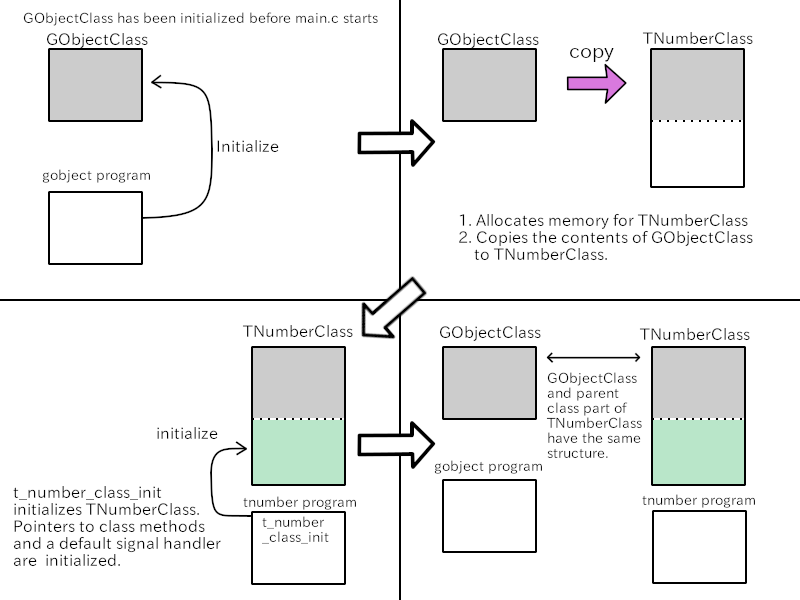
\includegraphics[width=12cm,height=9cm]{../image/tnumberclass_init.png}
\caption{TNumberClass initialization}
\end{figure}

\subsubsection{Initialization process of
TIntClass}\label{initialization-process-of-tintclass}

\begin{enumerate}
\def\labelenumi{\arabic{enumi}.}
\tightlist
\item
  TNumberClass has been initialized before the initialization of
  TIntClass starts.
\item
  First call for
  \passthrough{\lstinline!g\_object\_new (T\_TYPE\_INT, ...)!}
  initializes TIntClass. And the initialization process is as follows.
\item
  Memory is allocated for TIntClass. TIntClass doesn't have its own
  area. Therefore its structure is the same as its parent class
  (TNumberClass).
\item
  The parent (TNumberClass) part of the class (This is the same as whole
  TIntClass) is copied from TNumberClass.
\item
  The class initialization function
  \passthrough{\lstinline!t\_int\_class\_init!} is called. It overrides
  class methods from TNumber, \passthrough{\lstinline!set\_property!}
  and \passthrough{\lstinline!get\_property!}.
\end{enumerate}

The diagram below shows the process.

\begin{figure}
\centering
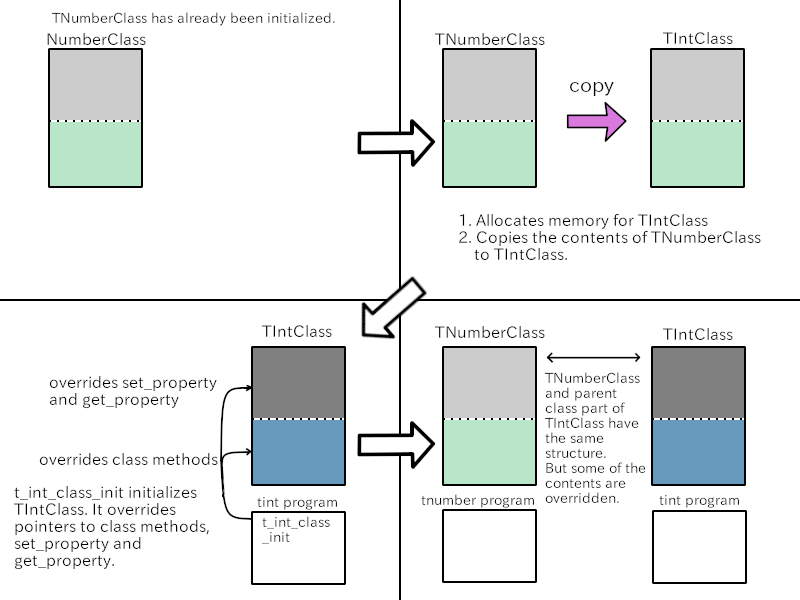
\includegraphics[width=12cm,height=9cm]{../image/tintclass_init.png}
\caption{TIntClass initialization}
\end{figure}
